\RequirePackage[l2tabu,orthodox]{nag}

% TODO: decide if one-sided/two-sided
%\documentclass[headsepline,footsepline,footinclude=false,fontsize=11pt,paper=a4,listof=totoc,bibliography=totoc,BCOR=12mm,DIV=12]{scrbook} % two-sided
\documentclass[headsepline,footsepline,footinclude=false,oneside,fontsize=11pt,paper=a4,listof=totoc,bibliography=totoc]{scrbook} % one-sided

\PassOptionsToPackage{table,svgnames,dvipsnames}{xcolor}

\usepackage[utf8]{inputenc}
\usepackage[T1]{fontenc}
\usepackage[sc]{mathpazo}
\usepackage[american]{babel}
\usepackage[autostyle]{csquotes}
\usepackage[%
  backend=biber,
  url=false,
  style=alphabetic,
  maxnames=4,
  minnames=3,
  maxbibnames=99,
  firstinits,
  uniquename=init]{biblatex} % TODO: adapt bibliography style
\usepackage{graphicx}
\usepackage{scrhack} % necessary for listings package
\usepackage{listings}
\usepackage{lstautogobble}
\usepackage{tikz}
\usepackage{pgfplots}
\usepackage{pgfplotstable}
\usepackage{booktabs}
\usepackage[final]{microtype}
\usepackage{caption}
\usepackage[hidelinks]{hyperref} % hidelinks removes colored boxes around references and links
\usepackage[toc,nonumberlist,acronym]{glossaries} % TODO: remove if glossary not needed

\bibliography{bibliography/literature}

\setkomafont{disposition}{\normalfont\bfseries} % use serif font for headings
\linespread{1.05} % adjust line spread for mathpazo font

% Settings for glossaries TODO: remove the following block if glossary not needed
\renewcommand{\glsnamefont}[1]{\normalfont\bfseries #1} % use serif font for glossary entry titles
\makeglossaries{}

% Settings for pgfplots
\pgfplotsset{compat=1.9} % TODO: adjust to your installed version
\pgfplotsset{
  % For available color names, see http://www.latextemplates.com/svgnames-colors
  cycle list={CornflowerBlue\\Dandelion\\ForestGreen\\BrickRed\\},
}

% Settings for lstlistings
\lstset{%
  basicstyle=\ttfamily,
  columns=fullflexible,
  autogobble,
  keywordstyle=\bfseries\color{MediumBlue},
  stringstyle=\color{DarkGreen}
}

% Basic information for cover & title page
\newcommand*{\getUniversity}{Technische Universität München}
\newcommand*{\getFaculty}{Department of Informatics}
\newcommand*{\getTitle}{TODO: Thesis title}
\newcommand*{\getTitleGer}{TODO: Titel der Abschlussarbeit}
\newcommand*{\getAuthor}{TODO: Author}
\newcommand*{\getDoctype}{TODO: Thesis type (Bachelor's Thesis in Informatics, Master's Thesis in Robotics, \ldots)}
\newcommand*{\getSupervisor}{TODO: Supervisor}
\newcommand*{\getAdvisor}{TODO: Advisor}
\newcommand*{\getSubmissionDate}{TODO: Submission date}
\newcommand*{\getSubmissionLocation}{Munich}

% TODO: add custom commands etc.


% TODO: remove if glossary not needed
\newglossaryentry{computer}
{
  name=computer,
  description={is a machine that\ldots}
}

\newacronym{tum}{TUM}{Technische Universität München}


\newcolumntype{R}[1]{>{\raggedleft\let\newline\\\arraybackslash\hspace{0pt}}m{#1}}

\begin{document}

\begin{titlepage}
  % HACK for two-sided documents: ignore binding correction for cover page.
  % Adapted from Markus Kohm's KOMA-Script titlepage=firstiscover handling.
  % See http://mirrors.ctan.org/macros/latex/contrib/koma-script/scrkernel-title.dtx,
  % \maketitle macro.
  \oddsidemargin=\evensidemargin\relax
  \textwidth=\dimexpr\paperwidth-2\evensidemargin-2in\relax
  \hsize=\textwidth\relax

  \centering

  
\includegraphics[width=40mm]{logos/tum}

  \vspace{5mm}
  {\huge\MakeUppercase{\getFaculty{}}}\\

  \vspace{5mm}
  {\large\MakeUppercase{\getUniversity{}}}\\

  \vspace{20mm}
  {\Large Secure Coding Phase 2}
  %{\Large \getDoctype{}}

  \vspace{15mm}
  %{\huge\bfseries \getTitle{}}

  \vspace{15mm}
  {\LARGE Team 3:
  	 Patrick Sattler, Aurel Roci, Stefan Kohler}
  %{\LARGE \getAuthor{}}

  \vspace{20mm}
  
\includegraphics[width=20mm]{logos/faculty}
\end{titlepage}


\frontmatter{}


{
	\chapter{Executive Summary}\
	We analyzed the white box texting report from team 9 that analyzed our web application in the last phase. We started by finding the vulnerabilities they found in our code and because most of them weren't as easy to fix as the ones we had in phase 4 we had to rewrite some parts of the web application. Additionally we have found additional bugs in our web application that team 9 never found and fixed them.
	
	The following chapters will guide you to the application architecture of our online banking solution, the security measures we used to make our app much more secure and finally the fixes we introduced in this phase for fixing the vulnerabilities found in the last phase.
	
	Our current state of the web application is much more secure than in the beginning of this lecture. We introduced many security measures that increase our web applications security. We are confident to provide a secure online banking solution.
}

\pagebreak
%\begin{titlepage}
  \centering

  
\includegraphics[width=40mm]{logos/tum}

  \vspace{5mm}
  {\huge\MakeUppercase{\getFaculty{}}}\\

  \vspace{5mm}
  {\large\MakeUppercase{\getUniversity{}}}\\
 
  \vspace{20mm}
  {\Large \getDoctype{}}

  \vspace{15mm}
  {\huge\bfseries \getTitle{}}

%  \vspace{10mm}
%  {\huge\bfseries \getTitleGer{}}

  \vspace{15mm}
%  \begin{tabular}{l l}
%    Author: & \getAuthor{} \\
%    Supervisor: & \getSupervisor{} \\
%    Advisor: & \getAdvisor{} \\
%    Submission Date: & \getSubmissionDate{} \\
%  \end{tabular}

  \vspace{20mm}
  
\includegraphics[width=20mm]{logos/faculty}
\end{titlepage}

%\thispagestyle{empty}
\vspace*{0.8\textheight}
\noindent
I confirm that this \MakeLowercase{\getDoctype{}} is my own work and I have documented all sources and material used.

\vspace{15mm}
\noindent
\getSubmissionLocation{}, \getSubmissionDate{} \hspace{5cm} \getAuthor{}

\cleardoublepage{}

%\addcontentsline{toc}{chapter}{Acknowledgments}
\thispagestyle{empty}

\vspace*{2cm}

\begin{center}
{\usekomafont{section} Acknowledgments}
\end{center}

\vspace{1cm}

%TODO: Acknowledgments

\cleardoublepage{}

%\chapter{\abstractname}

%TODO: Abstract



\microtypesetup{protrusion=false}
\tableofcontents{}
\microtypesetup{protrusion=true}
\mainmatter{}

\chapter{Time Tracking Table}

\begin{table}[htb]

	\centering
	\resizebox{9cm}{!}{%
	\begin{tabular}{lll}
		\hline
		{\textbf{Name}} & { \textbf{Task}} & {\textbf{Time}} \\ \hline
		Aurel Roci & Test File Extensions Handling for Sensitive Information and documenting & 1\\

		\hline
		\hline
		Stefan Ch. Kofler & Reverse-Engineer the binary file & 10\\
		& Binary-equivalent & 9 \\
		& Decompile jar file & 1 \\
	 
		
	\end{tabular}%
}
\end{table}

%\chapter{Introduction}\label{chapter:introduction}

\section{Section}
Citation test~\parencite{latex}.

\subsection{Subsection}
See~\autoref{fig:sample}.

\begin{figure}[htpb]
  \centering
  
\includegraphics{logos/tum}
  \caption[Example figure]{An example for a figure.}\label{fig:sample}
\end{figure}

\section{Section}

See~\autoref{tab:sample}, \autoref{fig:sample-drawing}, \autoref{fig:sample-plot}, \autoref{fig:sample-listing}.

\begin{table}[htpb]
  \caption[Example table]{An example for a simple table.}\label{tab:sample}
  \centering
  \begin{tabular}{l l l l}
    \toprule
      A & B & C & D \\
    \midrule
      1 & 2 & 1 & 2 \\
      2 & 3 & 2 & 3 \\
    \bottomrule
  \end{tabular}
\end{table}

\begin{figure}[htpb]
  \centering
  % This should probably go into a file in figures/
  \begin{tikzpicture}[node distance=3cm]
    \node (R0) {$R_1$};
    \node (R1) [right of=R0] {$R_2$};
    \node (R2) [below of=R1] {$R_4$};
    \node (R3) [below of=R0] {$R_3$};
    \node (R4) [right of=R1] {$R_5$};

    \path[every node]
      (R0) edge (R1)
      (R0) edge (R3)
      (R3) edge (R2)
      (R2) edge (R1)
      (R1) edge (R4);
  \end{tikzpicture}
  \caption[Example drawing]{An example for a simple drawing.}\label{fig:sample-drawing}
\end{figure}

\begin{figure}[htpb]
  \centering

  \pgfplotstableset{col sep=&, row sep=\\}
  % This should probably go into a file in data/
  \pgfplotstableread{
    a & b    \\
    1 & 1000 \\
    2 & 1500 \\
    3 & 1600 \\
  }\exampleA
  \pgfplotstableread{
    a & b    \\
    1 & 1200 \\
    2 & 800 \\
    3 & 1400 \\
  }\exampleB
  % This should probably go into a file in figures/
  \begin{tikzpicture}
    \begin{axis}[
        ymin=0,
        legend style={legend pos=south east},
        grid,
        thick,
        ylabel=Y,
        xlabel=X
      ]
      \addplot table[x=a, y=b]{\exampleA};
      \addlegendentry{Example A};
      \addplot table[x=a, y=b]{\exampleB};
      \addlegendentry{Example B};
    \end{axis}
  \end{tikzpicture}
  \caption[Example plot]{An example for a simple plot.}\label{fig:sample-plot}
\end{figure}

\begin{figure}[htpb]
  \centering
  \begin{tabular}{c}
  \begin{lstlisting}[language=SQL]
    SELECT * FROM tbl WHERE tbl.str = "str"
  \end{lstlisting}
  \end{tabular}
  \caption[Example listing]{An example for a source code listing.}\label{fig:sample-listing}
\end{figure}

% TODO: add more chapters here

\chapter{Application Architecture} \

Our applications consists of multiple files, most of them represent an own page in the web application, others are files that are included in this pages that perform some actions (e.g. creating a new user etc) and two models for the transactions and the users.

\section{Models}

We start by showing an UML class diagram of our two models.

\begin{figure}[!ht]
	\centering
	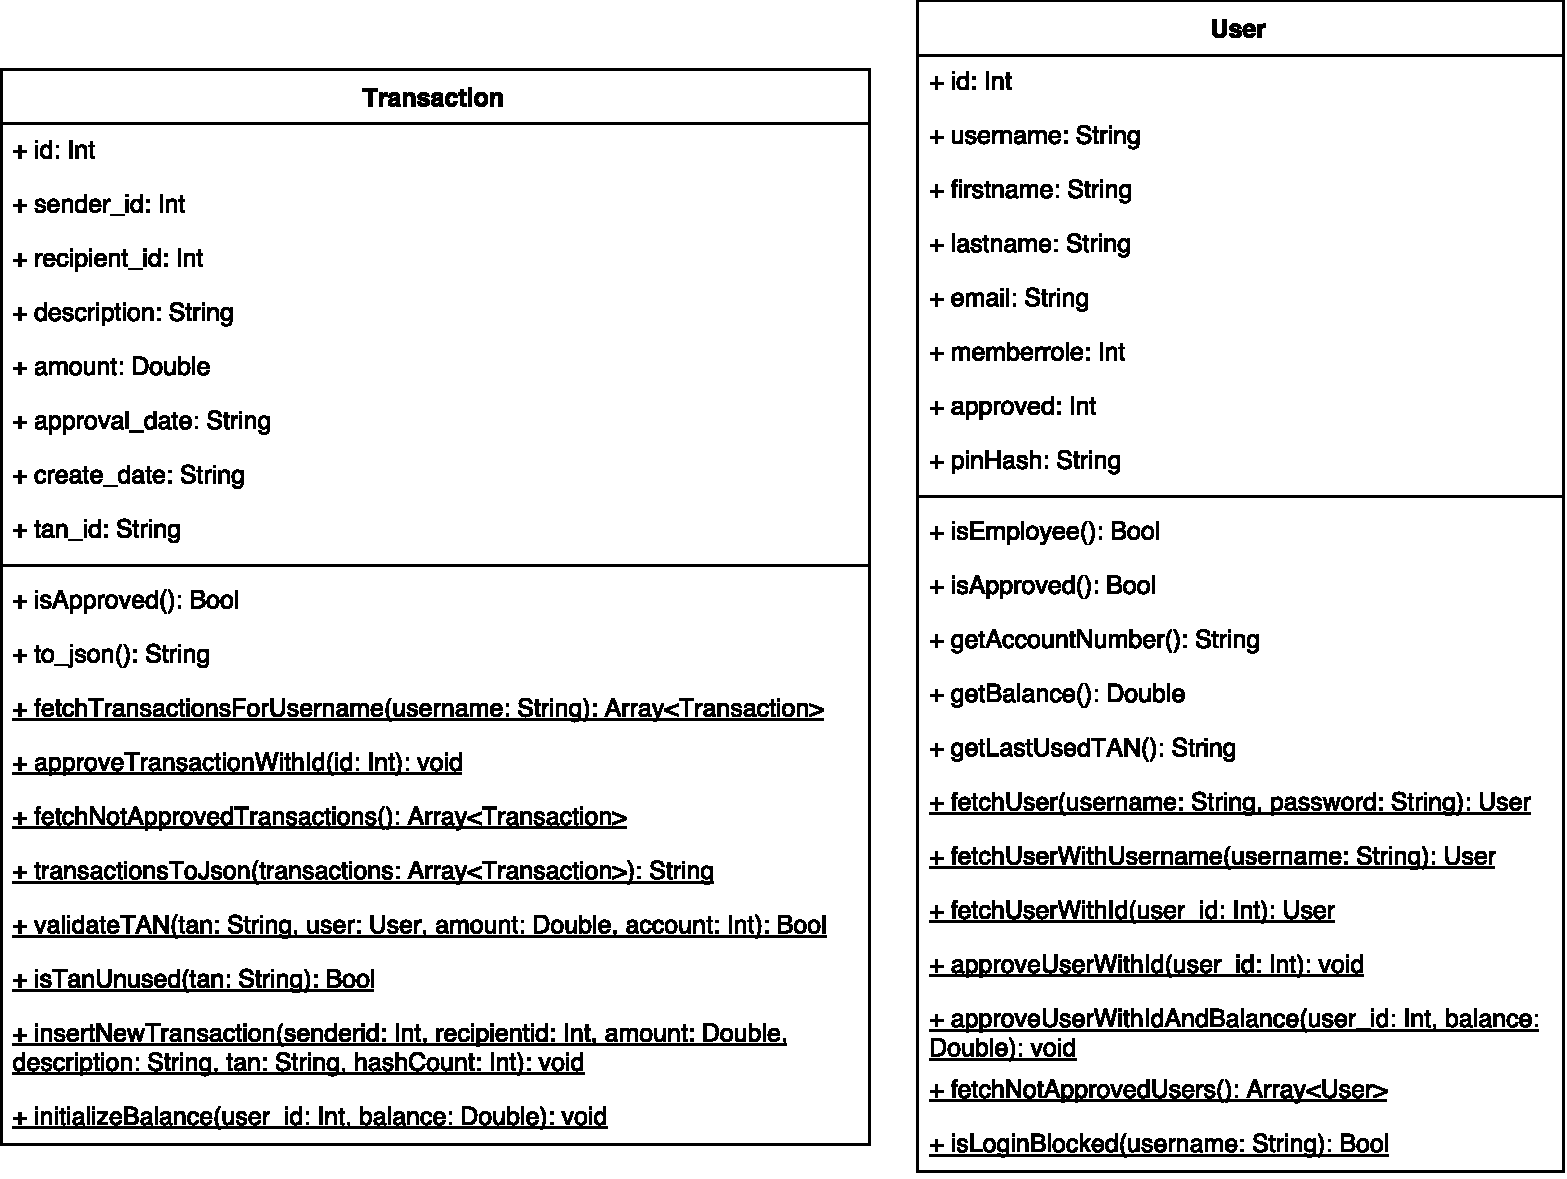
\includegraphics[scale=0.55]{figures/class_diagram.pdf}
	\caption{UML class diagram}
	\label{fig1}
\end{figure}

\subsection{Transaction}

An \textit{Transaction} object represents a single transaction. It contains all the necessary attributes that are also in the database table for the transactions. When fetching transaction from the database, these transactions are then mapped to \textit{Transaction} objects.

The class has also two helper methods for checking if an \textit{Transaction} is approved and to map it to JSON string.

Additionally the class has multiple class methods for fetching transactions, approving them, validating and checking TAN numbers, creating new transactions and to create a transaction that represents the initialization of a new user account with an specific balance.

\subsection{User}

\textit{User} objects represent an user account. It stores all the attributes of an user like their name, email address etc. This model gets also mapped from the database when fetching existing users.

This class some helper methods for detecting if the user is an employee, if the account is approved, to get the account number in the right format, to get the current balance of the user and to get his last used TAN number.

The \textit{User} class also has some class methods for fetching users, approving them and checking if the login system is blocked for this user.

\pagebreak

\section{Pages}

\begin{figure}[!ht]
	\centering
	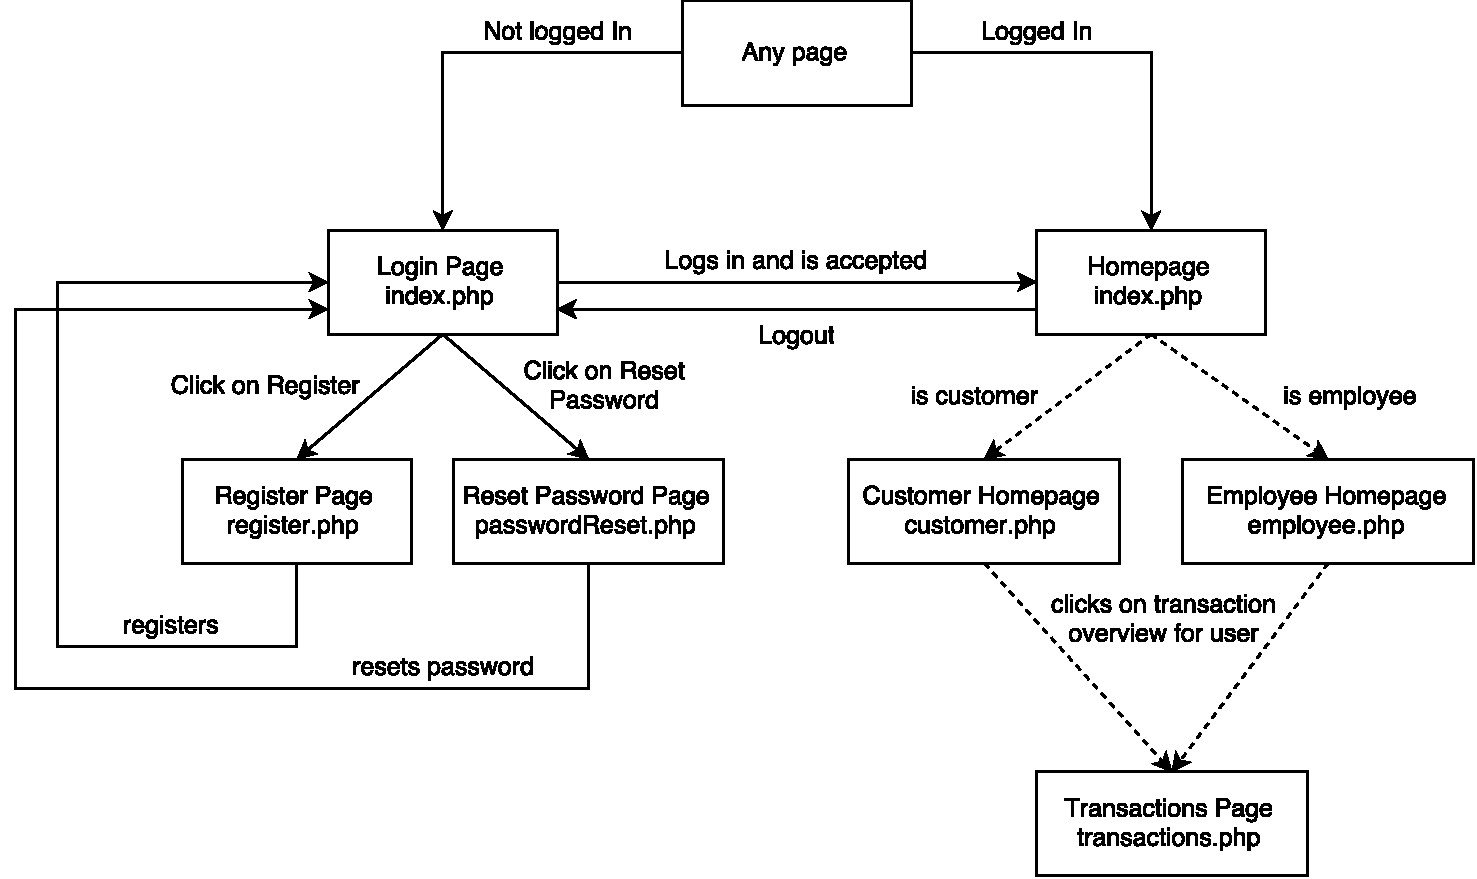
\includegraphics[scale=0.6]{figures/pages.pdf}
	\caption{Overview of different accessible pages}
	\label{pages}
\end{figure}

\autoref{pages} shows an overview of all the different accessible web pages and the flow between them.

It starts by the user accessing any page of the web application. If the user isn't logged in already he gets redirected to the login page otherwise to the homepage of his user role.

In the login page the user can log himself in, register a new account or reset his password. For the last two methods he gets redirected to an specific webpage for registering/resetting the password.

After logging in the system detects if the user account is the one of an customer or an employee and loads the corresponding PHP file. They have different functionality but both of the include the same \textit{transactions.php} file for showing the transaction overview for a specific user.

The functionality of these pages is mostly in different php files with the suffix .inc. These files are included in the pages PHP file and perform the necessary tasks a user clicked on.

The \textit{core.inc.php} file is included in all the web pages and provides some additional functionality needed in the web pages.

The \textit{init.sec.php} file is there to check on every page request if the user is logged in and prevents clickhijacking on the client side by adding some javascript to the web pages.

\pagebreak

\section{Frameworks}

The web application uses multiple external frameworks for providing functionality that would have been to much work to reimplement them on our own.

\subsection{Bootstrap}

\textit{Bootstrap} is a very popular HTML, CSS, and JS framework for developing user interfaces on the web. It helped us to build a great looking web application without spending to much time on the User Interface but rather on functionality and security.
The framework is available for free under the MIT license.

\subsection{jspdf}

We used \textit{jspdf} to deliver pdf's to the client for their transaction history. It is an easy to use client-side javascript framework that builds the pdf files on the fly without having them to be stored on the web server. That makes our web application more space efficient.

\subsection{fpdf}

For the TAN's that had to be sent as an password protected pdf over email we used the \textit{fpdf} framework. This framework is an pure PHP framework and not an javascript framework such as jspdf. It is also really easy to use and provides a lot of functionality. We used a second pdf framework because the requirements changed for phase 3 and jspdf wouldn't even have the option to create password protected PDF files.

\subsection{PHPMailer}

\textit{PHPMailer} is the framework of our choice for sending emails over PHP. It is full-featured and allowed us to send emails and even add attachments to the emails (for the generated TAN pdf files).

\pagebreak

\section{Interaction with other systems}

Our web service interacts with just one other system and that is the \textit{Gravatar} service for getting a profile picture for the user without storing it on the web server.

\textit{Gravatar} could be a potential security risk because the server isn't in our hands and if \textit{Gravatar} would be hacked, they could find out our users email addresses or could send instead of the profile picture other pictures that could lead to misuse of the online banking application.

It should be mentioned that it is a very small security risk and that is not comparable to sites using \textit{Google Analytics} and similar tools and some online banking solutions even use them. \textit{Gravatar} a useful service and is completely free.

\pagebreak
\section{Hardware/Software mapping}

\begin{figure}[!ht]
	\centering
	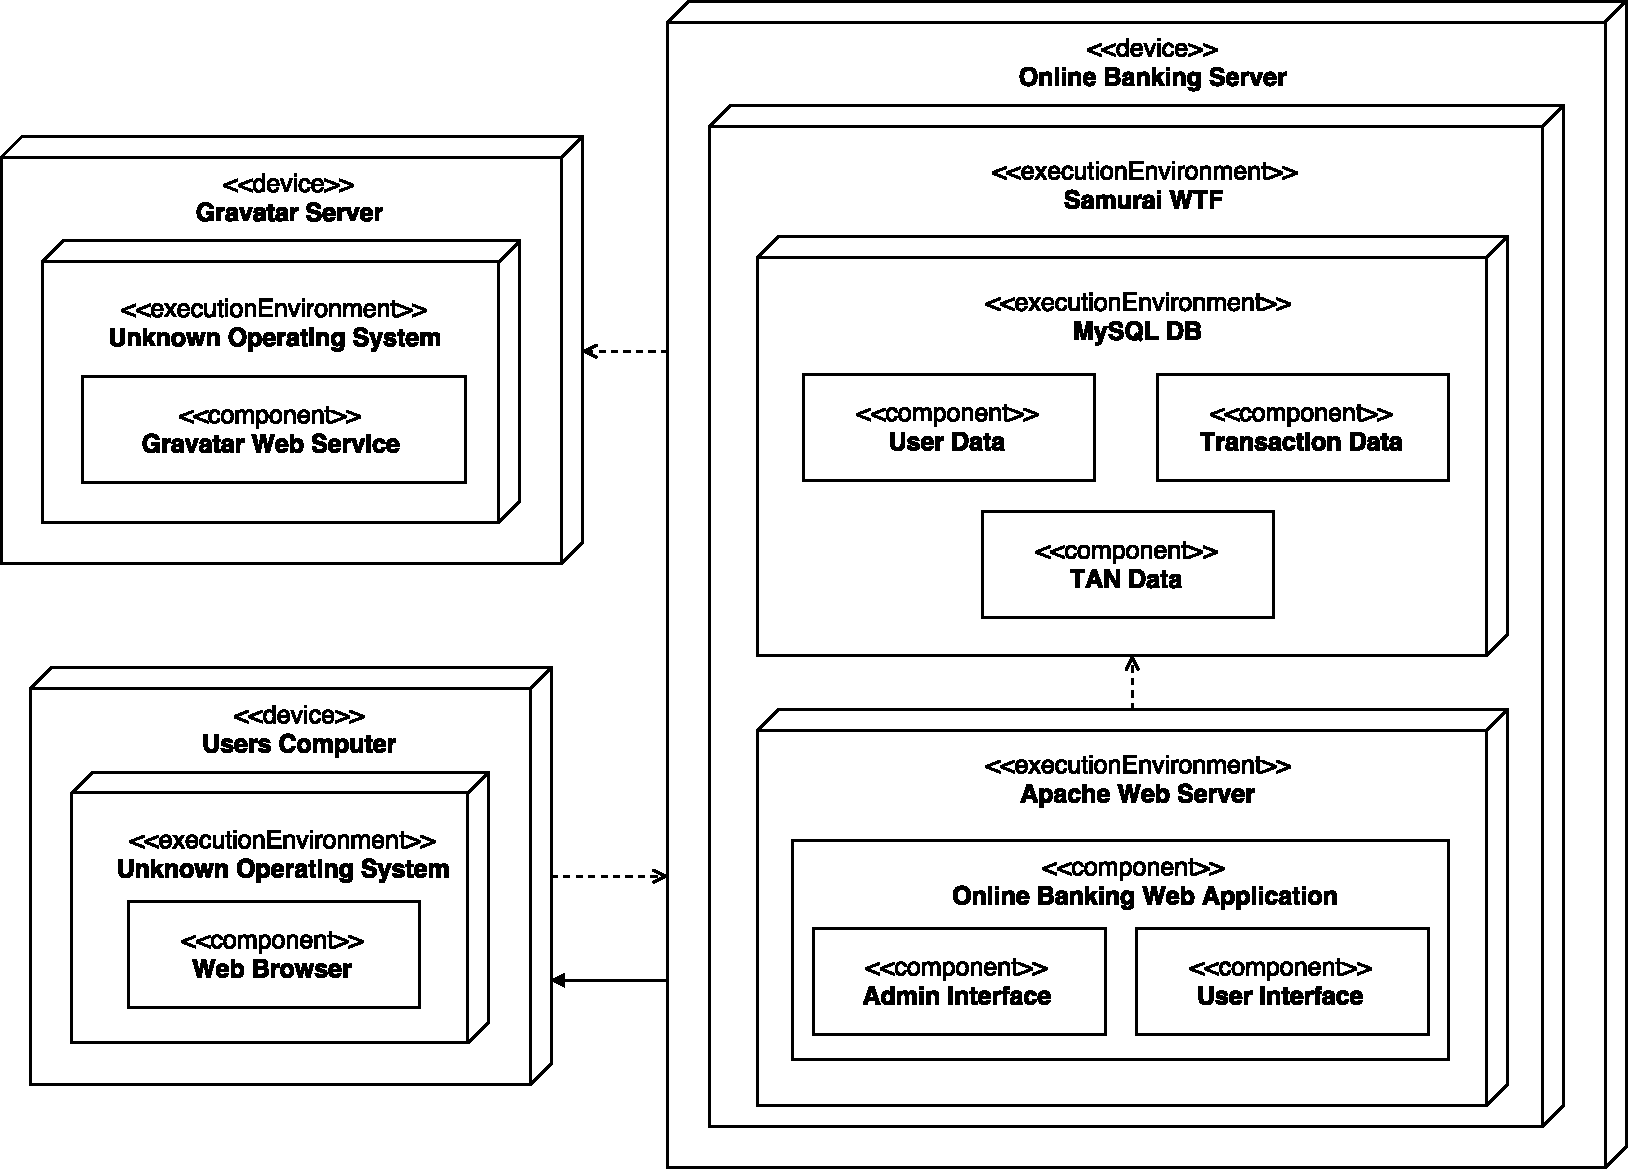
\includegraphics[scale=0.55]{figures/hw_sw_mapping.pdf}
	\caption{Hardware/Software Mapping (UML deployment diagram)}
	\label{fig1}
\end{figure}

Our online banking web application runs on an device called \textit{Online Banking Server} that is on our case a virtualized machine. This machine runs \textit{Samurai WTF} as an operation system. On this system we have two major services running. First the \textit{MySQL DB} database that contains the \textit{User Data}, \textit{Transaction Data}, and \textit{TAN Data}. On the other hand we have our \textit{Apache Web Server} on which our \textit{Online Banking Web Application} written in PHP is running. The web application has two major components: The \textit{Admin Interface} and the \textit{User Interface}.

\chapter{Security Measures}   
\subparagraph{Access Control}\

To access Standard Chartered Online Banking, you need a unique combination of Username and PIN. We have also introduced these additional measures to protect your account:

$\bullet$ Limited repeated attempts to login.\

$\bullet$ Automatic log out if there is no activity for a period of time. You will need to log in again if you wish to continue with the service.

\subparagraph{Encryption technology}\ 

The information exchanged between your Web browser and Online Banking is encrypted for your protection. Online Banking uses only \textit{https} requests between the Web Browser and server. This prevents attackers from doing a  Man-in-the-Middle attack.


\subparagraph{Password hashing}\

The Online Banking system uses password hashing to store passwords of accounts, that way only the user knows the password. We SHA256, considered as secure hash function, to hash the passwords into the database of Online Banking system. This prevents any attacker retrieving the passwords in case they gain access to the database.

\subparagraph{Password protected TANs}\

Upon registration the user, based on choice, receives an email with a password protected pdf file containing the TANs. The \textit{fpdf} library is used to generate this file, and the \textit{PHPMalier} library to send the email through an \textit{gmail} account.

\subparagraph{Personal PIN SCS}\

The Smart Card Simulator has a unique personal pin number for every user which is send to the user through email. The SCS uses SHA256 hash function to generate a hash that will be applied to the transaction section in the Online Banking system and compared to another hash for verification. The hash function is considered secure therefore the usage of the application for transactions is secure. Without the knowledge of the hashing key the attacker cannot generate hash to make transactions.

\subparagraph{Input sanitation}\

Every input made in the Online Banking system is controlled by PHP built-in functions (\textit{mysql\_real\_escape\_string}; \textit{htmlspecialchars}; \textit{escapeshellarg}...). This prevents any malicious input made by a user resulting in crashing the system, as well prevents any code injection done by an attacker. 

\subparagraph{Password Reset}\

In case the user wants to change the password of their account, they can make a request and then a link is send to their email, where they can change their password. This prevents any accidental change of password without the users knowledge.


\chapter{Fixes}

\subsection{Testing for Weak lock out mechanism(OTG-AUTHN-003)}\
After 3 wrong attempts to login the account now is blocked and an employee has now to approve it, for the user to be able to login. \

\textit{online\_banking/models/user.php} lines 177-178:\\

\begin{lstlisting} 
$query = "UPDATE users SET approved = 0 WHERE 
                 username='".mysql_real_escape_string($username)."';"; 
$result = mysql_query($query);
\end{lstlisting} 
After the user tries to log 3 times and fails the account will be blocked until an employee approves it again. So if the attacker deletes the session and tries again the account is blocked.\\


\subsection{Testing Directory traversal/file include (OTG-AUTHZ-001)}\

Fixed by fixing Command Injection and Local File Inclusion

\pagebreak
\subsection{Testing for bypassing authorization schema (OTG-AUTHZ-002)}\

\textit{online\_banking/register.php}, lines 130-157. Added a boolean function to check if less than two values are true.
\textit{online\_banking/init.sec.php}, lines 12-17, 
\begin{lstlisting}
$url = $_SERVER['REQUEST_URI'];

$isOnIndexPage = strpos($url, '/index.php') !== false;
$isOnRegisterPage = strpos($url, '/register.php') !== false;
$isOnEmployeePage = strpos($url, '/employee.php') !== false;
$isOnPasswordResetPage = strpos($url, '/passwordReset.php') !== false;
\end{lstlisting} 
and lines 27-32. 
\begin{lstlisting}
if (checkIfLessThanTwoBoolsAreTrue($isOnIndexPage, $isOnRegisterPage, $isOnEmployeePage, $isOnPasswordResetPage) == false) {
header('HTTP/1.0 400 Bad Request');
echo('This request is not valid!');
die();
}
\end{lstlisting} 
Added url variables and then check if less than two of this variables are true. If more then one is true send a bad request header and close the application.
\pagebreak
\subsection{Testing for Cross Site Request Forgery(OTG-SESS-005)}\
Added a new class that checks for the Csrf Token, \textit{online\_banking/CsrfToken.php}.
Added checks for the Csrf Token in the following files \textit{online\_banking/customer.inc.php} line 7 and line 11:
\begin{lstlisting}
7: $c = new \Csrf\CsrfToken(); 
11: if($post && $c->checkToken($timeout=300))
\end{lstlisting} 
\textit{online\_banking/employee.php}
\begin{lstlisting}
4: $c = new \Csrf\CsrfToken();
7: if($post && $c->checkToken($timeout=300))
17: else if (isset($_POST['user_id'])) 
25: $newToken = $c->generateToken();
130:  $randomString = $c->randomString();
133:  id="<?= $randomString ?>">
389: var params = "transaction_id="+id+"&csrf="+$_SESSION['csrf']['salt'];
\end{lstlisting} 
\textit{online\_banking/init.sec.php}
\begin{lstlisting}
12: require 'CsrfToken.php';
\end{lstlisting} 
\textit{online\_banking/login.inc.php}
\begin{lstlisting}
3: $c = new \Csrf\CsrfToken();
5: if($post && $c->checkToken($timeout=300)) {
29: <?php echo $c->generateHiddenField(); ?>
\end{lstlisting} 
\textit{online\_banking/passwordReset.inc.php}
\begin{lstlisting}
7: $c = new \Csrf\CsrfToken();
8: if($post && $emailSet && $c->checkToken($timeout=300)) 
42:  else if ($post && $idSet && $c->checkToken($timeout=300))
\end{lstlisting}
\textit{online\_banking/passwordReset.php}
\begin{lstlisting}
4: $c = new \Csrf\CsrfToken();
26: $hiddenField = $c->generateHiddenField();
30: <?php echo $hiddenField; ?>
65: <?php echo $hiddenField; ?>
\end{lstlisting}
\textit{online\_banking/register.inc.php}
\begin{lstlisting}
5: $c = new \Csrf\CsrfToken();
6: echo $c->checkToken($timeout=300) ? 'true' : 'false';
8: if ($c->checkToken($timeout=300))

\end{lstlisting}
\textit{online\_banking/register.php}
\begin{lstlisting} 
49: <?php echo $c->generateHiddenField(); ?>
\end{lstlisting}

\textit{online\_banking/transactions.php}
\begin{lstlisting} 
1: <?php
2: $c = new \Csrf\CsrfToken();
3: $hiddenField = $c->generateHiddenField();
4: ?>
10: <?php echo $hiddenField; ?>
60: <?php echo $hiddenField; ?>
\end{lstlisting}

\pagebreak
\subsection{Test Session Timeout(OTG-SESS-007)}\

Added a functionality in \textit{online\_banking/init.sec.php} in lines 17-21 :  


\begin{lstlisting}
(isset($_SESSION['LAST_ACTIVITY']) && (time() - $_SESSION['LAST_ACTIVITY'] > 900)) { 
session_unset();    
session_destroy();   
}
\end{lstlisting} 


This checks the last activity done in the website. If there is no activity for 15 minutes then the session is destroyed.\\



\subsection{Testing for Reflected Cross Site Scripting(OTG-INPVAL-001)} \

Insert a code in line 77 of the\textit{ online\_banking/employee.php} : 
\begin{lstlisting}
$search = htmlspecialchars($search);  

\end{lstlisting}
and line 54 of \textit{online\_banking/passwordReset.php}:  
\begin{lstlisting} 
htmlspecialchars($_GET['id']) 
\end{lstlisting}
to sanitize the input, so no code can be executed.
\pagebreak
\subsection{Testing for Stored Cross Site Scripting(OTG-INPVAL-002)}\
Insert code in lines 17 of \textit{online\_banking/customer.inc.php} to sanitized the input from XSS with the following code:   

\begin{lstlisting} 
$description = htmlspecialchars($description);
\end{lstlisting}

Changed the code in line 22 of \textit{online\_banking/register.inc.php} from :

\begin{lstlisting} 
    if(preg_match("/^$passwordRegex/", $password))
    to:
    if(preg_match("/^$emailRegex/", $email))
\end{lstlisting}
There was an if statement that checked for the password written twice, and we changed one to check for the email.\\



\subsection{Testing for SQL Injection (OTG-INPVAL-005) and Mysql testing (OTG-INPVAL-005)}\
Modified the query in line 131 of the \textit{online\_banking/models/user.php} file to sanitize the input: 
  
\begin{lstlisting} 
$query = "UPDATE users SET approved = 1 WHERE 
                       id='".mysql_real_escape_string($user_id)."';";
\end{lstlisting}
Also we sanitized the input in lines 137-140:

\begin{lstlisting}
$user_id = mysql_real_escape_string($user_id); 
$balance = mysql_real_escape_string($user_id);
$user_id = htmlspecialchars($user_id);
$balance = htmlspecialchars($balance);
\end{lstlisting}

This should prevent \textit{SQL Injections}.\\

\pagebreak
\subsection{Testing for Code Injection, Testing for Local File Inclusion, Testing for Remote File Inclusion(OTG-INPVAL-012)}\


Inserted a function when we read the variable in \textit{online\_banking/applicationDownload.php} line 2 :  

\begin{lstlisting} 
$user_id = intval($_GET['user_id']);
\end{lstlisting} 
to receive only integer values.
This will prevent any code injections.\\

\subsection{Testing for Command Injection(OTG-INPVAL-013)}\
Inserted code in line 3 of the \textit{online\_banking/applicationDownload.php} : 

\begin{lstlisting} 
$user_id = escapeshellarg($user_id);
\end{lstlisting}

 This way the shell commands are removed from the variable\\
 

\subsection{Testing for incubated vulnerabilities(OTG-INPVAL-015)}\
This vulnerability was fixed by fixing XSS, SQL Injection, Code Injection, Command Injection.
 
 
\subsection{Analysis of Error Codes (OTG-ERR-001)}\

Changed the PHP \textit{error\_reporting()} such that it does not display any errors: \textit{online\_banking/init.sec.php}; \textit{online\_banking/customer.sec.php}\\

\pagebreak
\subsection{Test Business Logic Data Validation(OTG-BUSLOGIC-001)}\

Added a server side check using regular expression in \textit{online\_banking/customer.sec.php} line 21: 
	\begin{lstlisting} 
	if($amount<0 || preg_match("/^$amountRegex/", $amount)) 
	\end{lstlisting}
	
	line 8:  
	
	\begin{lstlisting} 
	$amountRegex = "^\d*\.?\d*$";
	\end{lstlisting}
	
This way the check for the amount of money to transfer is server-side too. This will prevent any input of incorrect amount, even if the client-side check is bypassed.\\

 
\subsection{Test Integrity Checks(OTG-BUSLOGIC-003)}\

Fixed by fixing Injection vulnerabilities.\\
 
 
\subsection{Testing for JavaScript Execution(OTG-CLIENT-002)}\
Fixed by fixing Injection vulnerabilities. \\

 
\subsection{Testing for HTML Injection(OTG-CLIENT-003)}\
Fixed by fixing Injection vulnerabilities.\\ 

\subsection{Testing for CSS Injection(OTG-CLIENT-005)}\
Fixed by fixing Injection vulnerabilities.

\subsection{Test remember password functionality(OTG-AUTHN-005)}\
\textit{online\_banking/loginform.inc.php} line 26:
\begin{lstlisting} 
      <form action="<?php echo $current_file; ?>" method="POST" autocomplete="off">
\end{lstlisting}\
\textit{online\_banking/register.php} line 46:
\begin{lstlisting} 
			<form class="form-horizontal" id="register-form" 
				action='register.php' method="POST" onsubmit="return
				validateFields(this);" autocomplete="off">
\end{lstlisting} 

To instruct the web browser to don't show the user the dialog for saving the password and autofilling the login fields we set the \textit{autocomplete} attribute to \textit{off}. \\

It is still to be mentioned that modern web browsers ignore this attribute because the browsers password management is generally seen as a net gain for security. Since users don't have to remember passwords that the browser stores for them, they are able to choose stronger passwords than they would otherwise.

\subsection{Testing for bypassing authorization schema(OTG-AUTHZ-002)}\
\textit{online\_banking/core.inc.php} lines 130-157:\\
Added \textit{checkIfLessThanTwoBoolsAreTrue(\$var1, \$var2, \$var3, \$var4)} method for checking if less than two bool variables are true of a list of 4 variables.\\

\textit{online\_banking/init.sec.php} lines 27-31:
\begin{lstlisting} 
  if (checkIfLessThanTwoBoolsAreTrue($isOnIndexPage, $isOnRegisterPage, 
  		$isOnEmployeePage, $isOnPasswordResetPage) == false) {
    header('HTTP/1.0 400 Bad Request');
    echo('This request is not valid!');
    die();
  }
\end{lstlisting} 

The vulnerability was caused by a logic error in our web application. We checked if a user is on a specific page by searching for its path in url, but because \textit{Apache} always loads the first file specified in an URL it was possible to add other file paths add the end of the URL. Our web application then searched for file paths in the URL that should be accessible for everyone like the \textit{index.php} file and found it, even when it wasn't the page that was loaded by the \textit{Apache} web server.

We fixed this vulnerability by checking if multiple URL checks give the result true. If thats the case the URL isn't seen as valid anymore and we return with a 400 error representing a bad request.

\subsection{Testing for Cross Site Request Forgery(OTG-SESS-005)}\
\textit{online\_banking/core.inc.php} lines 13:\\
Remove session id regeneration after each request. We still keep the regeneration after a login and logout.\\

\textit{online\_banking/CsrfToken.php}:\\
New file from \textit{Github} for creating csrf tokens: \url{https://github.com/foxbunny/CSRF4PHP}\\

\textit{online\_banking/customer.inc.php} lines 7 and 11:\\
Create new \textit{CSRFToken} object and check if passed token is valid next to the check if it's a POST request.
\begin{lstlisting} 
  if($post && $c->checkToken($timeout=300))
\end{lstlisting} 

\textit{online\_banking/employee.php} lines 4, 7 and 389:\\
Adds csrf token checks\\

\textit{online\_banking/int.sec.php} line 12:\\
Imports CSRFToken.php file\\

\textit{online\_banking/loginform.inc.php} lines 3-5 and 29:\\
Adds csrf token checks\\

\textit{online\_banking/passwordReset.inc.php} lines 7-8 and 42:\\
Adds csrf token checks\\

\textit{online\_banking/passwordReset.php} lines 4, 26, 30 and 65:\\
Adds csrf token checks\\

\textit{online\_banking/register.inc.php} lines 5-6:\\
Adds csrf token checks\\

\textit{online\_banking/register.php} lines 5 and 49:\\
Adds csrf token checks\\

\textit{online\_banking/transactions.php} lines 1-5, 10 and 60:\\
Adds csrf token checks\\

\end{document}
